\documentclass[11pt]{article}

% ============================================================
% PACCHETTI
% ============================================================
\usepackage[a4paper, margin=2.5cm]{geometry}
\usepackage[utf8]{inputenc}
\usepackage[T1]{fontenc}
\usepackage{amsmath, amssymb}
\usepackage{graphicx}
\usepackage{booktabs}
\usepackage{array}
\usepackage{hyperref}
\usepackage{natbib}
\usepackage{setspace}
\usepackage{titlesec}
\usepackage{enumitem}
\usepackage{xcolor}

% The report figures can be uploaded to final_images_report/ on Overleaf.
\graphicspath{{final_images_report/}{outputs_multiseed/figures/}{outputs/figures/}{figures/}}

\hypersetup{
    colorlinks=true,
    linkcolor=blue,
    citecolor=blue,
    urlcolor=blue,
    pdftitle={How Much Data Is Enough for Meaningful Text-CNN Explanations?}
}

\title{How Much Data Is Enough for Meaningful Text-CNN Explanations?\\
\large A data-scaling and LIME analysis of sentiment classification on IMDB}
\author{Andrea Mauro\\Course: Machine learning for NLP}
\date{August 4, 2026}

\begin{document}

\maketitle

\begin{abstract}
This report investigates how the amount of supervised experience affects both the predictive performance and the apparent explanatory behavior of a fixed Text-CNN. The model is trained on the IMDB sentiment dataset using six nested, class-balanced training fractions: 1\%, 5\%, 10\%, 25\%, 50\%, and 100\%. The experiment is repeated with three random seeds (42, 123, and 2024), with the same protocol and hyperparameters in every run. Accuracy and macro-F1 are measured on a test set fixed within each seed, and results are reported as means and standard deviations across seeds. LIME explanations are generated for 100 balanced test reviews per seed and for every training fraction. The main quantitative interpretability measure is the proportion of stopwords and punctuation among the five most salient LIME tokens. The aggregated results show a clear learning curve: mean accuracy increases from 63.44\% $\pm$ 6.08\% with 1\% of the training data to 88.75\% $\pm$ 0.21\% with the full training set. The mean shortcut rate decreases from 77.60\% $\pm$ 7.50\% to 23.27\% $\pm$ 0.61\%, although it does not disappear. A minimal deletion test further shows that removing LIME's top-five tokens lowers the original-class probability on average in every condition. The report interprets these results in relation to Buckner's discussion of data requirements, human-like learning, and explanations in deep learning. It also argues that Buckner's treatment of nativism and empiricism is concentrated on perceptual and strategic domains, leaving socio-emotional cognition and sensorimotor grounding underdeveloped.
\end{abstract}

\tableofcontents
\newpage

% ============================================================
% PARTE 1 -- RESEARCH DESIGN
% ============================================================
\section{Research Design}
\label{sec:research-design}

\subsection{Research Question}

The research question is:

\begin{quote}
How does increasing the amount of supervised training data affect the predictive performance and the LIME-based explanatory behavior of a fixed Text-CNN trained for sentiment classification on IMDB reviews?
\end{quote}

This question is falsifiable because it defines a controlled independent variable, namely the fraction of the training set, and observable dependent variables: test accuracy, macro-F1, and the proportion of surface-level tokens among the most salient LIME features. The experiment is not only interested in whether a model becomes more accurate. It also asks whether additional data changes the type of evidence that the model appears to use.

The distinction is important because a classifier can achieve high accuracy by exploiting regularities that are predictive in the dataset but do not correspond to the semantic content of a review. For example, it may rely on sentiment-bearing adjectives, but it may also rely on punctuation, frequent function words, formatting patterns, or recurring stylistic conventions. A performance curve alone cannot distinguish these possibilities. The proposed experiment therefore combines a conventional learning curve with an explanation-based shortcut measure.

The central hypothesis is that performance will improve as the amount of training data increases and will eventually approach a plateau. A second hypothesis is that explanations will become less dependent on stopwords and punctuation. A stronger version of the second hypothesis would predict that the model will increasingly identify content words that directly express evaluation, such as \texttt{excellent}, \texttt{boring}, \texttt{terrible}, or \texttt{wonderful}. A possible alternative outcome is that accuracy will converge while shortcut reliance remains substantial. This would show that predictive success and semantically satisfactory explanations are related but not equivalent properties.

\subsection{Background and Motivation}

The design is motivated by the question of how much experience deep learning systems require in comparison with human learners. Buckner's discussion of this issue focuses on the large number of examples used by successful deep networks and asks whether their learning process is meaningfully similar to human learning \citep[Section 4.2]{buckner2019}. ImageNet systems and game-playing systems such as AlphaGo or AlphaZero provide striking examples of data-intensive learning, but they do not directly address text classification or the quality of explanations.

The IMDB dataset provides a useful controlled setting. It contains natural-language movie reviews labelled as positive or negative, so the task is a supervised form of linguistic and affective categorization. The dataset is not a direct test of theory of mind or human emotion recognition. Nevertheless, sentiment classification is closer to a social and evaluative domain than the closed strategic environments that dominate the nativism and empiricism debate in Buckner's Section 4.1.

The model used here is a Text-CNN. Text-CNNs apply convolutional operations over sequences of word embeddings and can detect local patterns such as short phrases. They are a natural text analogue of the convolutional architectures discussed by Buckner, although a Text-CNN is not identical to a visual DCNN. The architecture follows the general sentence-classification approach introduced by Kim \citep{kim2014}.

The second motivation comes from explainable artificial intelligence. LIME constructs a local surrogate model around a particular prediction by perturbing the input and learning which features are associated with the output \citep{ribeiro2016}. LIME does not provide a transparent view of the model's internal representation. It provides a local, post-hoc approximation. This limitation makes it especially useful for the present question: the experiment does not claim to measure semantic understanding directly, but measures whether the model's local explanations change as training data increases.

\subsection{Model Description}

The model is a binary Text-CNN classifier. Each review is converted into a sequence of tokens. Tokens are mapped to trainable embedding vectors, and several convolutional layers detect local n-gram patterns. A max-pooling operation keeps the strongest activation for each filter. The pooled features are concatenated and passed to a dropout layer and a linear classifier.

Let a tokenized review be represented as:

\begin{equation}
x = (x_1, x_2, \ldots, x_T),
\end{equation}

where $T$ is the maximum sequence length. Each token $x_i$ is mapped to an embedding vector $e_i \in \mathbb{R}^{d}$. For a convolutional kernel of width $k$, a local feature is computed as:

\begin{equation}
h_i^{(k)} = \operatorname{ReLU}\left(W^{(k)} e_{i:i+k-1} + b^{(k)}\right).
\end{equation}

The maximum value across all valid positions produces one pooled feature for the filter:

\begin{equation}
c^{(k)} = \max_i h_i^{(k)}.
\end{equation}

The vectors produced by the different kernel widths are concatenated:

\begin{equation}
c = [c^{(3)}; c^{(4)}; c^{(5)}].
\end{equation}

After dropout, the classifier produces two logits, one for the negative class and one for the positive class. A softmax converts the logits into class probabilities. Training minimizes the cross-entropy loss:

\begin{equation}
\mathcal{L}(\theta) = -\frac{1}{N}\sum_{i=1}^{N}\log p_{\theta}(y_i \mid x_i).
\end{equation}

In intuitive terms, a convolutional filter can learn to respond to a short sequence such as a positive adjective, a negative expression, or a recurring stylistic pattern. Max pooling makes the classifier sensitive to whether a pattern appears somewhere in a review without requiring it to appear at a fixed position.

\subsubsection{Architecture}

The architecture is fixed for all training fractions:

\begin{table}[htbp]
\centering
\caption{Fixed Text-CNN architecture.}
\label{tab:architecture}
\begin{tabular}{ll}
\toprule
Component & Configuration \\
\midrule
Vocabulary & 20,000 entries including padding and unknown tokens \\
Maximum sequence length & 400 tokens \\
Embedding dimension & 100 \\
Convolution widths & 3, 4, and 5 \\
Filters per width & 100 \\
Activation & ReLU \\
Pooling & Global max pooling \\
Dropout & 0.5 \\
Output & Two-class linear classifier \\
\bottomrule
\end{tabular}
\end{table}

For each seed, the vocabulary is constructed once from that seed's complete training pool, without using validation or test reviews, and is shared by the six models trained for that seed. This choice keeps the input representation and the number of parameters fixed across fractions within each seed. The fraction manipulation therefore changes the number of supervised examples used to update the model, rather than simultaneously changing the tokenizer or vocabulary size. The vocabulary and split can differ between seeds.

\subsubsection{Training Data and Procedure}

The source file is \texttt{IMDB Dataset.csv}, which contains 50,000 reviews and two sentiment labels. HTML markup is removed from the reviews, while ordinary words, stopwords, and punctuation are preserved. Preserving punctuation is necessary because punctuation is one of the possible surface-level features examined by the explanation analysis.

For each seed, the dataset is divided using a stratified split:

\begin{table}[htbp]
\centering
\caption{Dataset split used within each seed.}
\label{tab:split}
\begin{tabular}{lrrr}
\toprule
Split & Size & Positive & Negative \\
\midrule
Training pool & 40,000 & 20,000 & 20,000 \\
Validation & 5,000 & 2,500 & 2,500 \\
Test & 5,000 & 2,500 & 2,500 \\
\bottomrule
\end{tabular}
\end{table}

Six nested subsets are sampled from the training pool. Every subset contains the same number of positive and negative examples, and smaller subsets are contained in larger subsets. The subsets contain 400, 2,000, 4,000, 10,000, 20,000, and 40,000 reviews respectively.

The optimizer is Adam with a learning rate of $10^{-3}$ and a batch size of 64. Training runs for a maximum of ten epochs. Early stopping is applied using validation loss with a patience of two epochs, and the best validation checkpoint is restored before test evaluation. The experiment was repeated with three random seeds: 42, 123, and 2024. All runs used the same architecture, hyperparameters, preprocessing protocol, and Apple MPS device. Seed 42 is the original run, while seeds 123 and 2024 provide robustness checks.

\subsection{Experimental Design}

The independent variable is the percentage of the training pool used for supervised learning. The six levels are 1\%, 5\%, 10\%, 25\%, 50\%, and 100\%. The test set is never used for model selection or training. It is fixed across all six fractions within each seed, but it differs between seeds.

The dependent variables are:

\begin{enumerate}[label=\arabic*.]
    \item Test accuracy.
    \item Test macro-F1.
    \item The proportion of stopwords among the five most salient LIME tokens.
    \item The proportion of punctuation tokens among the five most salient LIME tokens.
    \item The combined proportion of stopwords and punctuation tokens.
    \item Qualitative changes in the semantic plausibility of the explanations.
\end{enumerate}

For the LIME analysis, 100 test reviews are selected for each seed: 50 positive and 50 negative reviews. The exact same 100 reviews are explained for all six fractions within a seed, while the sample can differ between seeds. Each LIME explanation uses 1,000 perturbed samples and targets the model's predicted class. The five tokens with the largest absolute LIME weights are stored. Thus, the multiseed analysis contains 300 examples and 1,500 top-five token observations per fraction.

For an example $j$, let $s_j$ be the number of stopwords among its top-five tokens and $p_j$ the number of punctuation tokens. The aggregate shortcut rate for a training fraction $f$ is:

\begin{equation}
SR_f = \frac{\sum_{j=1}^{N}(s_j+p_j)}{5N}.
\end{equation}

This measure is deliberately operational rather than semantic. Stopwords and punctuation are not always meaningless. For example, exclamation marks can express emphasis and function words can participate in useful constructions. The metric should therefore be interpreted as reliance on surface-level token classes, not as a proof that every flagged token is noise.

\subsection{Predicted Outcomes and Interpretation}

The expected learning curve is monotonic or approximately monotonic: models trained on more reviews should generalize better to the test set used within each seed. The largest gains are expected at the smallest fractions because the 1\% model has very little supervised experience. Performance should eventually plateau as the model receives enough examples to learn the dominant sentiment regularities.

If the shortcut rate decreases together with accuracy, this would suggest that additional data helps the model move from generic surface cues toward more content-sensitive features. If the shortcut rate remains constant, the result would indicate that more data improves prediction without changing the type of local evidence exposed by LIME. If the shortcut rate increases, the model may be learning a highly predictive stylistic regularity that is reinforced by the larger training set.

The strongest interpretation would require more than the present experiment. A lower shortcut rate does not establish human-like understanding, and LIME's weights are not a causal account of the neural computation. The intended conclusion is more modest: the data-scaling curve can reveal whether predictive learning and explanation-level surface reliance improve at the same rate.

\subsection{Limitations}

The experiment uses three random seeds, which provides a basic estimate of variability but is not enough to support very broad claims about all possible initializations or data splits. The 1\% condition shows substantially more variation than the larger fractions, especially for accuracy and macro-F1.

Within each seed, the shared vocabulary is constructed from the complete training pool. This controls the architecture and avoids confounding the six fractions with different vocabularies, but it means that the 1\% condition benefits from a tokenizer built using text from the larger training pool. Labels are not used in vocabulary construction, yet this preprocessing choice should be reported as a limitation.

The IMDB labels are review-level sentiment labels. They do not measure emotion recognition, theory of mind, intention, or social norm learning. The dataset is therefore only a limited bridge between ordinary sentiment classification and socio-emotional cognition.

LIME is a local surrogate method and its explanations can be unstable. The shortcut metric is also dependent on the selected stopword list, tokenization scheme, number of features, and fixed test sample. Finally, the model is text-only and has no sensorimotor interaction with the world. It cannot by itself test whether linguistic representations are grounded in the sense proposed by Eliasmith.

\newpage

% ============================================================
% PARTE 2 -- PAPER REVIEW
% ============================================================
\section{Paper Review}
\label{sec:paper-review}

\subsection*{Paper reviewed}

Buckner, C. (2019). \textit{Deep learning: A philosophical introduction}. \textit{Philosophy Compass}, e12625. DOI: \url{https://doi.org/10.1111/phc3.12625}.

\subsection{Summary}

Buckner's article introduces deep learning to readers in philosophy of mind and philosophy of science. Its central claim is that contemporary deep convolutional neural networks deserve separate philosophical attention rather than being treated as merely larger versions of the shallow connectionist networks discussed in the 1980s and 1990s. The paper combines a technical explanation of DCNNs with an analysis of what their success may imply about learning, abstraction, intelligence, and scientific explanation.

The introductory section presents deep learning as a major shift in artificial intelligence. Buckner points to achievements in image recognition, speech, translation, scientific prediction, and game playing. He also emphasizes that the success of these systems is philosophically important because their performance exceeds earlier expectations while their relation to human intelligence remains unsettled.

Section 2 explains the principal architectural properties of DCNNs. Depth allows networks to compose simple transformations into more complex functions. Heterogeneity combines convolution, rectification, and pooling rather than relying on a single type of unit. Sparse connectivity reduces the number of parameters and reflects local receptive fields. Regularization, including dropout and early stopping, limits overfitting. The section's purpose is not merely descriptive: Buckner argues that these properties produce computational advantages that distinguish DCNNs from older shallow networks.

Section 3 examines three explanations for the success of deep networks. The first is hierarchical feature composition, according to which later layers build increasingly abstract features from simpler ones. The second is systematic transformation of input to handle nuisance variation, such as position, pose, rotation, pitch, or duration. The third concerns the large number of linear regions that deep networks can create in input space. Buckner presents these explanations as potentially complementary rather than mutually exclusive.

Section 4 turns to philosophical questions. In the discussion of nativism and empiricism, Buckner analyses claims that systems such as AlphaZero vindicate learning from experience. He uses Marcus's variables $a$, $r$, $k$, and $e$ to distinguish algorithms, representational formats, innate knowledge, and experience. AlphaZero is not a pure blank slate because it includes rules, search procedures, and structural assumptions. In the discussion of human-like learning, Buckner considers the number of examples required by DCNNs and the significance of adversarial examples. The final subsection asks what kind of explanation DCNNs provide: mechanistic, functional, mathematical, or some combination of these.

\subsection{Strengths}

The paper's main strength is its ability to connect technical details with philosophical questions without treating the technical details as irrelevant implementation choices. The explanations of depth, convolution, pooling, sparse connectivity, and regularization give the reader enough background to understand why deep networks differ from shallow networks.

The discussion of AlphaZero is also valuable because it avoids a simplistic interpretation of success as evidence for a completely blank-slate learner. Buckner distinguishes learned strategy from built-in rules, search mechanisms, and domain-general assumptions. This distinction makes the empiricism debate more precise than the common claim that self-play eliminates all innate structure.

Another strength is the treatment of competing explanations. Hierarchical abstraction, nuisance-variable adjustment, and linear-region capacity are not presented as a single magical explanation for deep learning. Instead, Buckner shows how different mathematical and architectural properties may contribute to the same empirical success.

The treatment of adversarial examples is especially relevant to the present experiment. High performance on naturally occurring examples does not guarantee that a network has acquired the same category knowledge as a human. This distinction between benchmark performance and the structure of learned representations provides a useful conceptual basis for examining whether accuracy and explanation quality converge together.

Finally, the paper is open about the limits of the analogy between DCNNs and biological systems. Buckner notes that the networks are abstract models of cortical processing and that the biological plausibility of backpropagation remains debated. This cautious attitude makes the paper suitable as a starting point for a critical review rather than only as a defense of deep learning.

\subsection{Critical Discussion}

\subsubsection*{The social and emotional domain is missing from the nativism debate}

The treatment of nativism and empiricism in Section 4.1 is intellectually useful, but its main examples are concentrated in strategic games and perceptual categorization. AlphaZero is an especially favorable case for an empiricist interpretation: the domain has explicit rules, a discrete action space, a clear success criterion, and an effectively unlimited source of self-play experience. This is not a neutral test of whether experience can replace domain-specific knowledge. It is a highly structured environment in which feedback is unusually clean.

The situation is different in social and emotional cognition. Recognizing an intention, interpreting an ambiguous facial expression, learning a social norm, or deciding whether an action was appropriate often involves uncertain and delayed feedback. The relevant categories may be context-dependent, and there may be no objective equivalent of winning a game. The classical literature on theory of mind, including \citet{baron1985}, and research on face perception, including \citet{kanwisher1997}, shows that the nativism debate has long included social and perceptual domains. Carey \citep{carey2009} also discusses candidate core concepts such as OBJECT, AGENT, NUMBER, and CAUSE. Buckner cites this tradition, but he does not develop its implications for deep learning models of agency, intention, or emotion.

This omission matters for the framework built around $a$, $r$, $k$, and $e$. In a socio-emotional task, it is unclear what should count as experience, what counts as a successful outcome, and which representational primitives are required before learning can begin. A system could receive many labelled examples and still fail to learn a robust concept if the labels do not capture the relevant social context. The fact that a model can fit sentiment labels on reviews does not settle this issue, because review sentiment is a relatively coarse and explicit target.

\subsubsection*{The absence of Eliasmith and sensorimotor grounding}

The paper also leaves out a literature that is closely related to its discussion of abstraction and adversarial examples. Eliasmith's Semantic Pointer Architecture and Neural Engineering Framework offer a perspective in which useful semantic representations are compressed but remain connected to the patterns from which they originate, including sensorimotor information \citep{eli2013}. This is not the same as claiming that every representation must preserve all raw sensory details. The important point is that abstraction should remain functionally and causally linked to embodied interaction.

This perspective could provide an alternative interpretation of adversarial examples. A network that is trained only to exploit statistical regularities in pixels or tokens can be highly accurate on ordinary inputs while remaining vulnerable to small, unnatural changes. A system grounded in an agent's sensorimotor interaction might instead be expected to rely more heavily on properties that are stable under action and causal intervention. Grounding would not automatically solve adversarial robustness, but it would shift the explanation away from the simple idea that the network has merely not seen enough examples.

The same issue arises in the present text experiment. A Text-CNN trained on reviews receives linguistic strings and labels, not bodily states, facial expressions, actions, or social consequences. Its learned representations may be useful for classification while remaining amodal statistical structures. LIME can reveal that the model's local decision is associated with a word or punctuation mark, but it cannot show that the model possesses the kind of grounded semantic pointer described by Eliasmith.

\subsubsection*{Explanation and faithfulness}

Buckner's final section asks what kind of explanation DCNNs provide, but the paper predates the widespread use of many practical post-hoc explanation pipelines in NLP. LIME is itself a useful example of the distinction between explaining a prediction and revealing the actual mechanism that generated it. Its local linear surrogate may be faithful in a small neighbourhood while failing to describe the model outside that neighbourhood. Consequently, a list of salient words should not automatically be treated as the model's true internal reasons.

The present experiment addresses this issue only partially. It compares explanation patterns across training-data conditions and records LIME's local surrogate score. A minimal deletion test is also included in the analysis: the five top-ranked tokens are removed and the change in the probability of the original predicted class is measured. This is a stronger test of local predictive influence than LIME weights alone, although it is not a complete causal account and does not yet include a random-token baseline.

\subsection{Relation to Broader Questions}

The article sits at the intersection of several broader debates. First, it revisits nativism and empiricism in a computational setting. Deep learning demonstrates that substantial structure can be acquired from experience, but it does not show that no structure is innate. Architectures, learning algorithms, representations, optimization procedures, and task definitions all impose prior constraints.

Second, the article concerns the relationship between symbolic and subsymbolic representation. DCNNs do not manipulate explicit rules in the classical symbolic sense, yet they can produce categorical and abstract behaviour. The open question is whether this abstraction is conceptually similar to human abstraction or only functionally adequate on a restricted distribution.

Third, the article contributes to the debate between mechanistic and functional explanation. A DCNN may offer a mathematical explanation of why a function can be computed efficiently, a functional explanation of what transformation is being performed, or a mechanistic explanation of a biological system. These explanatory roles should not be conflated.

The current experiment adds a fourth connection: data scaling and explanation scaling. If more examples increase accuracy but do not consistently improve local explanations, this would support a distinction between learning a decision boundary and learning a representation that appears semantically organized. It would also provide a text-based complement to Buckner's discussion of whether deep networks learn in a human-like way.

\subsection{Open Questions for Further Discussion}

\begin{enumerate}[label=(\alph*)]
    \item The nativism/empiricism debate in Buckner's Section 4.1 is developed mainly through perceptual and logical-strategic tasks such as ImageNet and Go. Does Marcus's framework of algorithms, representational formats, innate knowledge, and experience apply equally well to socio-emotional cognition, or would it require substantial modifications because social feedback is ambiguous and lacks a single objective success metric?
    \item Do the DCNNs discussed by Buckner provide genuine sensorimotor grounding, or do they remain amodal representations expressed as numerical vectors? More specifically, could the absence of grounding help explain the adversarial vulnerabilities discussed in Section 4.2, rather than treating those vulnerabilities only as a consequence of insufficient training data?
\end{enumerate}

\newpage

% ============================================================
% PARTE 3 -- ANALYSIS
% ============================================================
\section{Analysis}
\label{sec:analysis}

\subsection*{Practical selected}

The practical selected is a custom data-scaling and explanation analysis on IMDB sentiment classification. Its original purpose is to study the relation between training-set size and model behaviour. The implementation extends this purpose by applying LIME to a fixed sample within each seed, quantifying the presence of stopwords and punctuation in the most salient features, and adding a minimal deletion test.

\subsection{Experimental Protocol}

The experiment was implemented in \texttt{run\_experiment.py}. The CSV was loaded with pandas, and the two sentiment labels were converted to binary values: negative equals 0 and positive equals 1. HTML tags were removed from the reviews, but punctuation was preserved.

For each seed, the complete dataset was split into a training pool, validation set, and test set using stratified sampling. The training pool contains 40,000 reviews, while validation and test each contain 5,000 reviews. The validation and test sets are fixed for all six fractions within a seed, but the split differs between seeds.

The training subsets were created by shuffling the positive and negative training examples separately and taking the same number from each class. Because the same shuffled class-specific order is reused, the subsets are nested. This ensures that the experiment varies the amount of training experience while avoiding a new class imbalance or a completely different sample composition at every fraction.

The Text-CNN uses a 20,000-entry vocabulary, 100-dimensional embeddings, 100 filters for each of the three convolution widths 3, 4, and 5, global max pooling, dropout of 0.5, and a two-class linear output layer. Adam is used with learning rate $10^{-3}$ and batch size 64. Each model is trained for at most ten epochs with early stopping patience two. The best validation checkpoint is used for test evaluation. Six models are trained for each seed, resulting in 18 model checkpoints overall.

For LIME, a balanced sample of 100 reviews is selected from the test set for each seed. The sample is saved in the corresponding output directory, such as \texttt{outputs/lime\_examples.csv} for seed 42 and \texttt{outputs\_seed123/lime\_examples.csv} for seed 123, and is reused for all six fractions within that seed. Each review is perturbed 1,000 times. The five tokens with the largest absolute local weights are stored in the corresponding \texttt{lime\_explanations.csv} file. A token is counted as a stopword if it belongs to the fixed English stopword list used by scikit-learn. It is counted as punctuation if it contains no alphanumeric characters. The combined shortcut rate is saved in the corresponding \texttt{lime\_summary.csv} file.

The minimal Deletion Test is implemented in \texttt{run\_deletion\_test.py}. For each seed, it reuses the six saved checkpoints and the existing LIME explanations. For each review, all occurrences of the five LIME token types are removed. The probability assigned to the model's original predicted class is measured before and after deletion. The probability drop is defined as:

\begin{equation}
\Delta p = p(\hat{y}\mid x) - p(\hat{y}\mid x \setminus T_5),
\end{equation}

where $\hat{y}$ is the original predicted class and $T_5$ is the set of LIME top-five token types. The test also records whether the predicted class changes after deletion. No model is retrained.

The original seed-42 run was performed in two stages. First, models were trained and evaluated with:

\begin{verbatim}
python3 run_experiment.py --skip-lime
\end{verbatim}

The saved checkpoints were then reused for LIME with:

\begin{verbatim}
python3 run_experiment.py --lime-only
\end{verbatim}

Finally, the minimal deletion analysis was run with:

\begin{verbatim}
python3 run_deletion_test.py
\end{verbatim}

This separation avoids unnecessary retraining when the explanation analysis is regenerated. Seeds 123 and 2024 were run through the complete pipeline using \texttt{run\_all\_seeds.sh}, followed by their deletion tests. Finally, \texttt{aggregate\_seeds.py} combined the three seed directories into \texttt{outputs\_multiseed/}.

\subsection{Results}

The quantitative results are shown in Table~\ref{tab:main-results}. Each seed evaluates its six models on a fixed 5,000-review test set. The table reports the mean $\pm$ standard deviation across the three seeds. For LIME, each seed contributes 500 top-token observations per fraction, giving 1,500 observations in the multiseed analysis.

\begin{table}[htbp]
\centering
\small
\caption{Predictive performance and LIME shortcut rates.}
\label{tab:main-results}
\resizebox{\textwidth}{!}{%
\begin{tabular}{rrrrrrr}
\toprule
Training & Examples & Accuracy & Macro-F1 & Stopword & Punctuation & Shortcut \\
fraction & & mean $\pm$ std & mean $\pm$ std & rate & rate & rate \\
\midrule
1\% & 400 & 63.44\% $\pm$ 6.08\% & 61.99\% $\pm$ 7.55\% & 53.20\% $\pm$ 6.01\% & 24.40\% $\pm$ 5.00\% & 77.60\% $\pm$ 7.50\% \\
5\% & 2,000 & 78.41\% $\pm$ 1.62\% & 78.34\% $\pm$ 1.58\% & 48.33\% $\pm$ 0.92\% & 15.20\% $\pm$ 5.33\% & 63.53\% $\pm$ 6.00\% \\
10\% & 4,000 & 82.32\% $\pm$ 0.21\% & 82.29\% $\pm$ 0.23\% & 44.00\% $\pm$ 4.92\% & 9.53\% $\pm$ 4.35\% & 53.53\% $\pm$ 2.39\% \\
25\% & 10,000 & 85.89\% $\pm$ 0.25\% & 85.88\% $\pm$ 0.25\% & 29.27\% $\pm$ 7.13\% & 7.47\% $\pm$ 0.61\% & 36.73\% $\pm$ 6.63\% \\
50\% & 20,000 & 87.61\% $\pm$ 0.59\% & 87.61\% $\pm$ 0.59\% & 21.27\% $\pm$ 2.20\% & 5.27\% $\pm$ 1.21\% & 26.53\% $\pm$ 3.41\% \\
100\% & 40,000 & 88.75\% $\pm$ 0.21\% & 88.75\% $\pm$ 0.21\% & 17.53\% $\pm$ 1.68\% & 5.73\% $\pm$ 2.16\% & 23.27\% $\pm$ 0.61\% \\
\bottomrule
\end{tabular}
}%
\end{table}

The predictive learning curve is strongly positive. Mean accuracy increases by 25.31 percentage points between the 1\% and 100\% conditions. The largest gains occur between 1\% and 5\%, while the difference between 50\% and 100\% is 1.14 percentage points. The standard deviation is also much larger at 1\% than at the larger fractions, indicating that the smallest training condition is more sensitive to the random seed.

The shortcut curve shows a similar but not identical pattern. Mean combined surface-token reliance decreases from 77.60\% at 1\% to 23.27\% at 100\%. It falls especially strongly between 25\% and 50\%. At 100\%, the remaining shortcut rate is driven mainly by stopwords rather than punctuation. The variability is largest at 1\% and 25\%, showing that explanation-level measures are also sensitive to the seed.

The mean LIME local-surrogate scores from the original seed-42 run are not monotonic: they are approximately 0.382, 0.620, 0.561, 0.498, 0.358, and 0.402 across the six fractions. These values are retained as a seed-42 illustration because the current multiseed aggregation does not include a pooled local-surrogate score. This result still shows that the amount of data does not automatically make LIME a better local approximation. The shortcut rate and the LIME surrogate score measure different properties.

The minimal Deletion Test provides an additional faithfulness diagnostic. For each review, all occurrences of the five LIME token types are removed, and the probability of the model's original predicted class is measured again. The results are shown in Table~\ref{tab:deletion-results}.

\begin{table}[htbp]
\centering
\small
\caption{Minimal Deletion Test results.}
\label{tab:deletion-results}
\begin{tabular}{rrr}
\toprule
Training & Mean probability & Prediction-flip \\
fraction & drop (mean $\pm$ std) & rate (mean $\pm$ std) \\
\midrule
1\% & 0.031 $\pm$ 0.013 & 23.0\% $\pm$ 3.0\% \\
5\% & 0.139 $\pm$ 0.026 & 24.3\% $\pm$ 3.8\% \\
10\% & 0.188 $\pm$ 0.003 & 22.0\% $\pm$ 1.7\% \\
25\% & 0.203 $\pm$ 0.026 & 18.0\% $\pm$ 2.6\% \\
50\% & 0.187 $\pm$ 0.027 & 20.3\% $\pm$ 4.2\% \\
100\% & 0.178 $\pm$ 0.031 & 14.3\% $\pm$ 2.1\% \\
\bottomrule
\end{tabular}
\end{table}

The probability drop is positive on average for every training fraction, indicating that the LIME top-five tokens are not merely arbitrary words. The mean probability drop increases from 0.031 at 1\% to a maximum of 0.203 at 25\%, then remains positive at 0.178 for the full training set. The prediction-flip rate decreases overall from 23.0\% at the smallest fraction to 14.3\% at the largest fraction, but the intermediate values are not monotonic. This suggests that larger-data models may become more robust to deleting a small set of salient tokens, possibly because they distribute evidence across redundant features or because their predictions are more confident. The deletion effect is not monotonic, so more data does not simply make the top-five explanation more causally concentrated. The aggregate files report the mean probability drop and flip rate; median drop and positive-drop rate were not pooled by the aggregation script and are therefore not included in this table.

The Deletion Test should still be interpreted cautiously. Removing all occurrences of a token type can alter the review substantially, especially for frequent stopwords. In addition, the test has no random-token control condition. Therefore, it establishes local sensitivity to the LIME-selected features, but not that those features are more influential than equally many randomly selected tokens.

\begin{figure}[htbp]
\centering
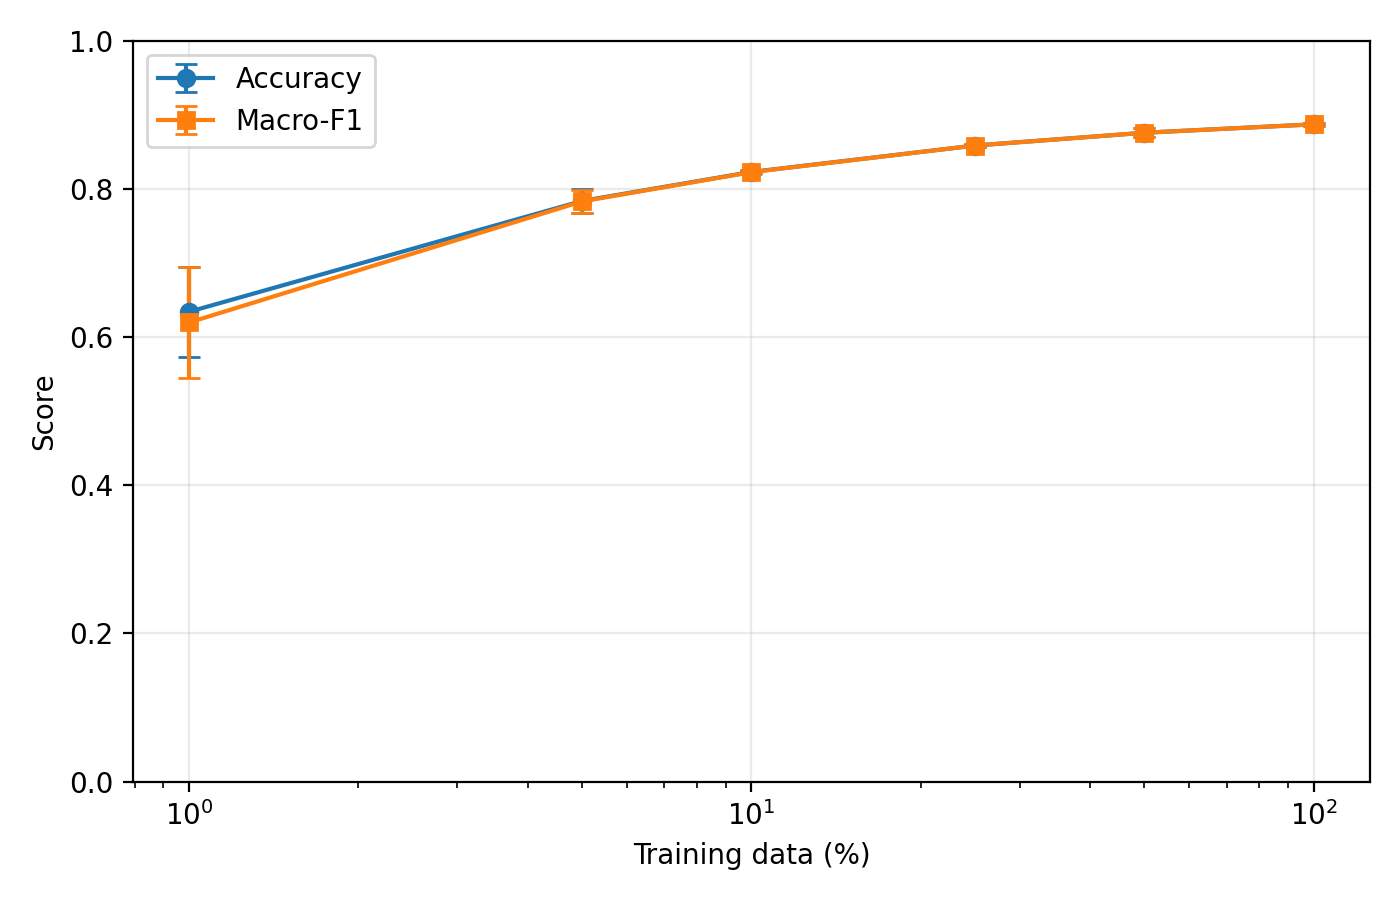
\includegraphics[width=0.82\textwidth]{final_images_report/learning_curve_meanstd.png}
\caption{Mean accuracy and macro-F1 as a function of the training fraction. Error bars show the standard deviation across the three seeds.}
\label{fig:learning-curve}
\end{figure}

\begin{figure}[htbp]
\centering
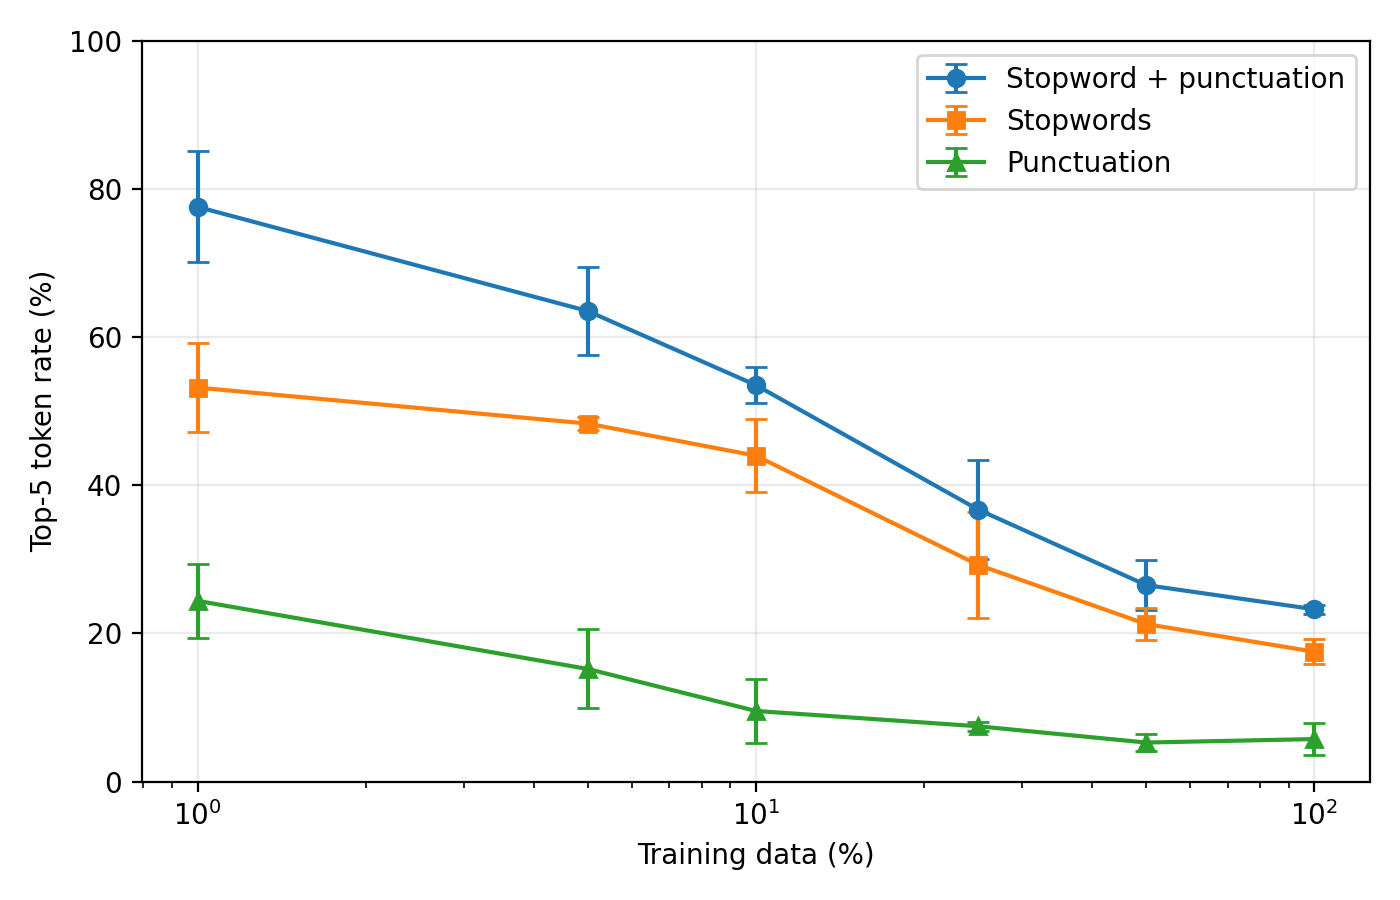
\includegraphics[width=0.82\textwidth]{final_images_report/lime_shortcuts_meanstd.png}
\caption{Mean stopword, punctuation, and combined shortcut rates among LIME top-five tokens. Error bars show the standard deviation across the three seeds.}
\label{fig:lime-shortcuts}
\end{figure}

\begin{figure}[htbp]
\centering
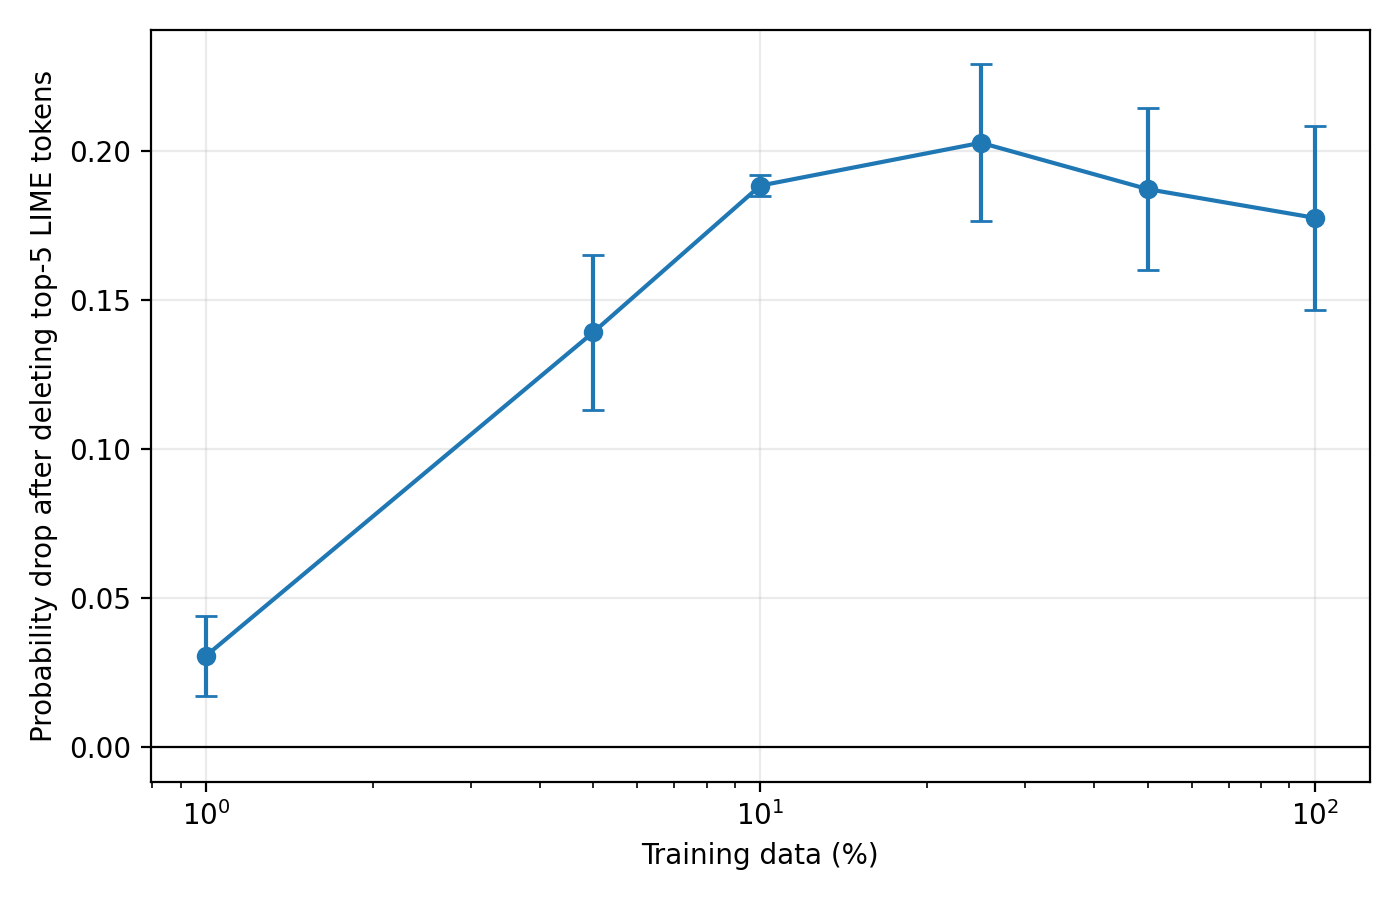
\includegraphics[width=0.82\textwidth]{final_images_report/deletion_drop_meanstd.png}
\caption{Mean probability drop after deleting LIME's top-five token types. Error bars show the standard deviation of the seed-level means across the three seeds.}
\label{fig:deletion}
\end{figure}

The qualitative explanations from the seed-42 sample illustrate a transition from generic or surface-level tokens toward more content-bearing words. For review 2047, the 1\% model selects punctuation and stopwords, while larger models increasingly select \texttt{worst}, \texttt{awful}, \texttt{wooden}, \texttt{lousy}, and \texttt{insult}. The true label is negative, and the model changes from an incorrect positive prediction at 1\% to a confident negative prediction at larger fractions.

For review 2467, the 1\% model again relies on \texttt{and}, while the 5\% and 10\% models begin to select \texttt{nothing} and \texttt{boring}. At 25\% and above, the explanations contain \texttt{terrible}, \texttt{boring}, \texttt{dull}, \texttt{disappointment}, and \texttt{script}. These terms are more directly related to the negative evaluation of the film.

For review 3709, which is a very short negative review, the 1\% explanation contains \texttt{been}, \texttt{I}, \texttt{so}, and punctuation. At larger fractions, \texttt{boring}, \texttt{ending}, \texttt{credits}, and \texttt{roll} become salient. These features reflect the actual content of the review more closely, although stopwords such as \texttt{to} and \texttt{see} remain present.

\begin{table}[htbp]
\centering
\small
\caption{Illustrative LIME trajectories for three reviews in the seed-42 sample.}
\label{tab:qualitative}
\begin{tabular}{p{0.12\textwidth}p{0.26\textwidth}p{0.26\textwidth}p{0.26\textwidth}}
\toprule
Review & 1\% explanation & 25\% explanation & 100\% explanation \\
\midrule
2047 & \texttt{,}, \texttt{.}, \texttt{an}, \texttt{"}, \texttt{that} & \texttt{worst}, \texttt{awful}, \texttt{effort}, \texttt{even}, \texttt{This} & \texttt{worst}, \texttt{insult}, \texttt{wooden}, \texttt{lousy}, \texttt{awful} \\
2467 & \texttt{,}, \texttt{and}, \texttt{were}, \texttt{off}, \texttt{some} & \texttt{terrible}, \texttt{boring}, \texttt{dull}, \texttt{nothing}, \texttt{and} & \texttt{terrible}, \texttt{dull}, \texttt{disappointment}, \texttt{script}, \texttt{and} \\
3709 & \texttt{been}, \texttt{glad}, \texttt{I}, \texttt{so}, \texttt{.} & \texttt{boring}, \texttt{see}, \texttt{ending}, \texttt{credits}, \texttt{roll} & \texttt{boring}, \texttt{credits}, \texttt{glad}, \texttt{to}, \texttt{see} \\
\bottomrule
\end{tabular}
\end{table}

The table is a qualitative illustration from seed 42 rather than an independently sampled statistical test or a multiseed aggregate. The complete quantitative result is represented by the multiseed shortcut-rate curve.

\subsection{Discussion}

The results support the first hypothesis: more supervised data improves generalization. The mean accuracy curve rises sharply at small fractions and then approaches a plateau. This is consistent with Buckner's observation that deep learning systems often require large quantities of experience to achieve strong benchmark performance. In the present experiment, models trained on only 400 reviews are substantially less reliable on average than models trained on 40,000 reviews.

The results also support the second hypothesis in a qualified form. The mean combined shortcut rate decreases from 77.60\% $\pm$ 7.50\% to 23.27\% $\pm$ 0.61\%. Therefore, increasing the amount of training data is associated not only with better predictions but also with a lower frequency of stopwords and punctuation in the top-five LIME features. The effect is especially strong between 25\% and 50\% of the training set, although the variability across seeds is greater at some smaller fractions.

However, the result is not that explanations become fully semantic. Even the 100\% condition assigns, on average, 17.53\% of its top-five features to stopwords and 5.73\% to punctuation. The mean shortcut rate decreases from 26.53\% at 50\% to 23.27\% at 100\%, but the standard deviations show that explanation patterns still vary across seeds. This illustrates that predictive convergence and explanation cleanliness do not have to be perfectly aligned.

The qualitative cases from seed 42 support the quantitative pattern, but they should not be interpreted as a statistical summary of all seeds. At 1\%, LIME often highlights function words or punctuation, and the model can be uncertain or wrong. With more data, content words associated with evaluation become more common in the explanations. Nevertheless, LIME still identifies stopwords in some high-data explanations. This is compatible with the interpretation that the model learns a mixture of semantic and surface regularities rather than replacing one with the other in a clean sequence.

The experiment provides a small text-based extension of Buckner's Section 4.2. It operationalizes training experience as the number of labelled reviews and asks whether increased experience makes the model's behaviour more human-interpretable. The answer is partly positive: additional data improves both accuracy and the selected surface-token measure. But the remaining shortcut reliance and the non-monotonic local-surrogate scores support a more cautious conclusion. More data can improve the decision boundary without guaranteeing a faithful or grounded explanation.

The experiment also connects to the critical discussion of socio-emotional cognition. Sentiment classification involves evaluative language, but it is still a simplified task with explicit labels and no interaction. It cannot determine whether a model learns concepts such as intention, agency, or emotion in the richer sense discussed in cognitive science. This limitation makes the experiment relevant to the open question, but not a solution to it.

The Deletion Test strengthens the interpretation of the LIME results without eliminating their limitations. The fact that removing the top-five tokens lowers the original-class probability on average in every condition suggests that the explanations have some local predictive relevance. At the same time, the mean flip rate is lower at 100\% than at 1\%, although it is not monotonic at intermediate fractions. This suggests that model confidence and robustness can increase even when LIME remains partly dependent on surface tokens. This is another example of why accuracy, explanation cleanliness, and explanation faithfulness should be reported as separate dimensions.

Finally, the results do not establish sensorimotor grounding. The model has no body, action policy, or perceptual stream. The fact that its LIME explanations become more content-sensitive at larger data scales does not show that its representations are grounded. From an Eliasmith-inspired perspective, the model may simply have learned more robust linguistic correlations while remaining an amodal classifier.

\subsection{Additional Explorations (optional but encouraged)}

The minimal Deletion Test is a completed extension of the original analysis. It measures probability changes after removing the LIME top-five token types for all six checkpoints within each of the three seeds. The multiseed aggregation improves the robustness of the main conclusions, while several further extensions would strengthen the analysis.

First, more than three independent random seeds could be used for each fraction. This would provide a more stable estimate of variability caused by initialization, subset sampling, and the different stratified splits.

Second, the shortcut analysis could be expanded beyond stopwords and punctuation. A part-of-speech tagger could distinguish content words from function words, and a named-entity recognizer could measure reliance on actor names, film titles, and locations. These measures would directly address the possibility that a model uses proper names or dataset-specific entities as shortcuts.

Third, the current Deletion Test should be extended with a random-token baseline and, ideally, an insertion test. The top LIME tokens could be compared with equally many randomly selected token types. This would test whether the salient tokens are more influential for the classifier than arbitrary tokens rather than merely plausible to a human reader.

Fourth, LIME could be compared with another attribution method, such as integrated gradients or SHAP. Agreement between methods would provide stronger evidence that the observed change in salient features is not an artefact of one explainer.

\subsection{Limitations}

The analysis uses three train-validation-test splits, one for each seed. The LIME sample contains 100 reviews per seed, which is adequate for a controlled comparison but not large enough to support broad claims about all IMDB reviews or natural language sentiment classification. Three seeds are also insufficient to characterize the full distribution of possible results.

The combined shortcut metric is intentionally simple. It treats all stopwords and punctuation as one surface category, even though some of these tokens can be meaningful. The qualitative analysis partly addresses this issue, but a richer linguistic annotation would be preferable.

The experiment measures LIME outputs, not the internal semantics of the model. The term ``explanation quality'' must therefore be used cautiously. The current results show changes in a post-hoc attribution pattern, not proof of a change in human-like understanding or grounding.

The Deletion Test is also limited. It removes all occurrences of each selected token type and has no random-token baseline. A positive probability drop therefore shows sensitivity to the selected features, but it does not prove that LIME identifies the uniquely or maximally influential features.

The IMDB dataset also has known stylistic regularities and may contain duplicate or near-duplicate patterns. A model that performs well on these test splits may not generalize to other review domains. Finally, the shared vocabulary within each seed improves experimental control but gives every fraction access to a vocabulary built from the larger training pool, so the experiment isolates supervised learning rather than total exposure to raw text.

\newpage

% ============================================================
% BIBLIOGRAFIA
% ============================================================
\begin{thebibliography}{99}

\bibitem[Baron-Cohen et al.(1985)]{baron1985}
Baron-Cohen, S., Leslie, A. M., and Frith, U. (1985).
Does the autistic child have a theory of mind?
\textit{Cognition}, 21(1), 37--46.

\bibitem[Buckner(2019)]{buckner2019}
Buckner, C. (2019).
Deep learning: A philosophical introduction.
\textit{Philosophy Compass}, e12625.
\url{https://doi.org/10.1111/phc3.12625}.

\bibitem[Carey(2009)]{carey2009}
Carey, S. (2009).
\textit{The Origin of Concepts}.
Oxford University Press.

\bibitem[Eliasmith(2013)]{eli2013}
Eliasmith, C. (2013).
\textit{How to Build a Brain: A Neural Architecture for Biological Cognition}.
Oxford University Press.

\bibitem[Kanwisher et al.(1997)]{kanwisher1997}
Kanwisher, N., McDermott, J., and Chun, M. M. (1997).
The fusiform face area: A module in human extrastriate cortex specialized for face perception.
\textit{The Journal of Neuroscience}, 17(11), 4302--4311.

\bibitem[Kim(2014)]{kim2014}
Kim, Y. (2014).
Convolutional neural networks for sentence classification.
In \textit{Proceedings of EMNLP 2014}, 1746--1751.

\bibitem[Lake et al.(2017)]{lake2017}
Lake, B. M., Ullman, T. D., Tenenbaum, J. B., and Gershman, S. J. (2017).
Building machines that learn and think like people.
\textit{Behavioral and Brain Sciences}, 40, e253.

\bibitem[Maas et al.(2011)]{maas2011}
Maas, A. L., Daly, R. E., Pham, P. T., Huang, D., Ng, A. Y., and Potts, C. (2011).
Learning word vectors for sentiment analysis.
In \textit{Proceedings of ACL 2011}, 142--150.

\bibitem[Marcus(2018a)]{marcus2018a}
Marcus, G. (2018a).
Deep learning: A critical appraisal.
arXiv:1801.00631.

\bibitem[Marcus(2018b)]{marcus2018b}
Marcus, G. (2018b).
Innateness, AlphaZero, and artificial intelligence.
arXiv:1801.05667.

\bibitem[Ribeiro et al.(2016)]{ribeiro2016}
Ribeiro, M. T., Singh, S., and Guestrin, C. (2016).
Why should I trust you? Explaining the predictions of any classifier.
In \textit{Proceedings of KDD 2016}, 1135--1144.

\end{thebibliography}

\end{document}
